\begin{frame}{\textit{Godot}}{Conceitos gerais}

\begin{figure}

\includegraphics[width=0.4\textwidth]{image/godot-logo.png}
\end{figure}

\begin{itemize}
\item Criação de Juan Linietsky e Ariel Manzur em 2007

\item Código aberto ao público em 2014

\item<2-> Código fonte escrito em \textbf{\textit{C\texttt{++}}}

\item<3-> Programação de jogos simplificada por meio de \textbf{\textit{GDScript}}
\end{itemize}
\end{frame}

% ---------------------------------------------------------------------

\begin{frame}{\textit{Godot}}{Classes importantes}

\begin{itemize}
\item \texttt{Object}: Classe base para todos os tipos não embutidos em \textit{Godot}

\item<2-> \texttt{Reference}: Gerenciamento automático de memória

\item<3-> \texttt{Resource}: Armazenamento de dados

\item<4-> \texttt{Node}: Define um comportamento
\end{itemize}

\uncover<5->{
\begin{figure}
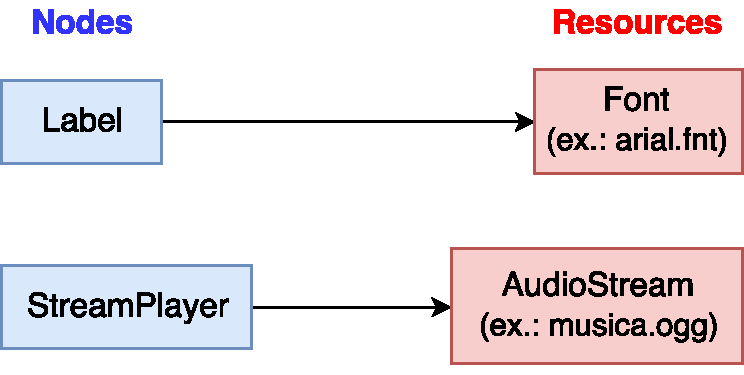
\includegraphics[width=0.5\textwidth]{image/resource.pdf}
\end{figure}
}
\end{frame}
